% https://medium.com/@pawan329/ocr-extract-text-from-image-in-8-easy-steps-3113a1141c34

\chapter{OCR: Extract Text from Image In 8 Easy Steps}

Intoday’s digital world, extracting text from images has become a crucial task in various applications, such as document digitization, text recognition, and data extraction. Python provides several powerful libraries that enable us to perform Optical Character Recognition (OCR) to extract text from images effortlessly. In this article, we will explore the process of extracting text from images using Python, focusing on the popular Tesseract OCR engine.

We’ll use Pytesseract to perform this task.
Pytesseract is an OCR library in Python that is used to extract text from images. Python-tesseract is a Python wrapper for Google’s Tesseract-OCR.

\section{Step 1. Install Tesseract on your machine}

Visit \URL{https://github.com/UB-Mannheim/tesseract/wiki} and download Tesseract installer for Windows.

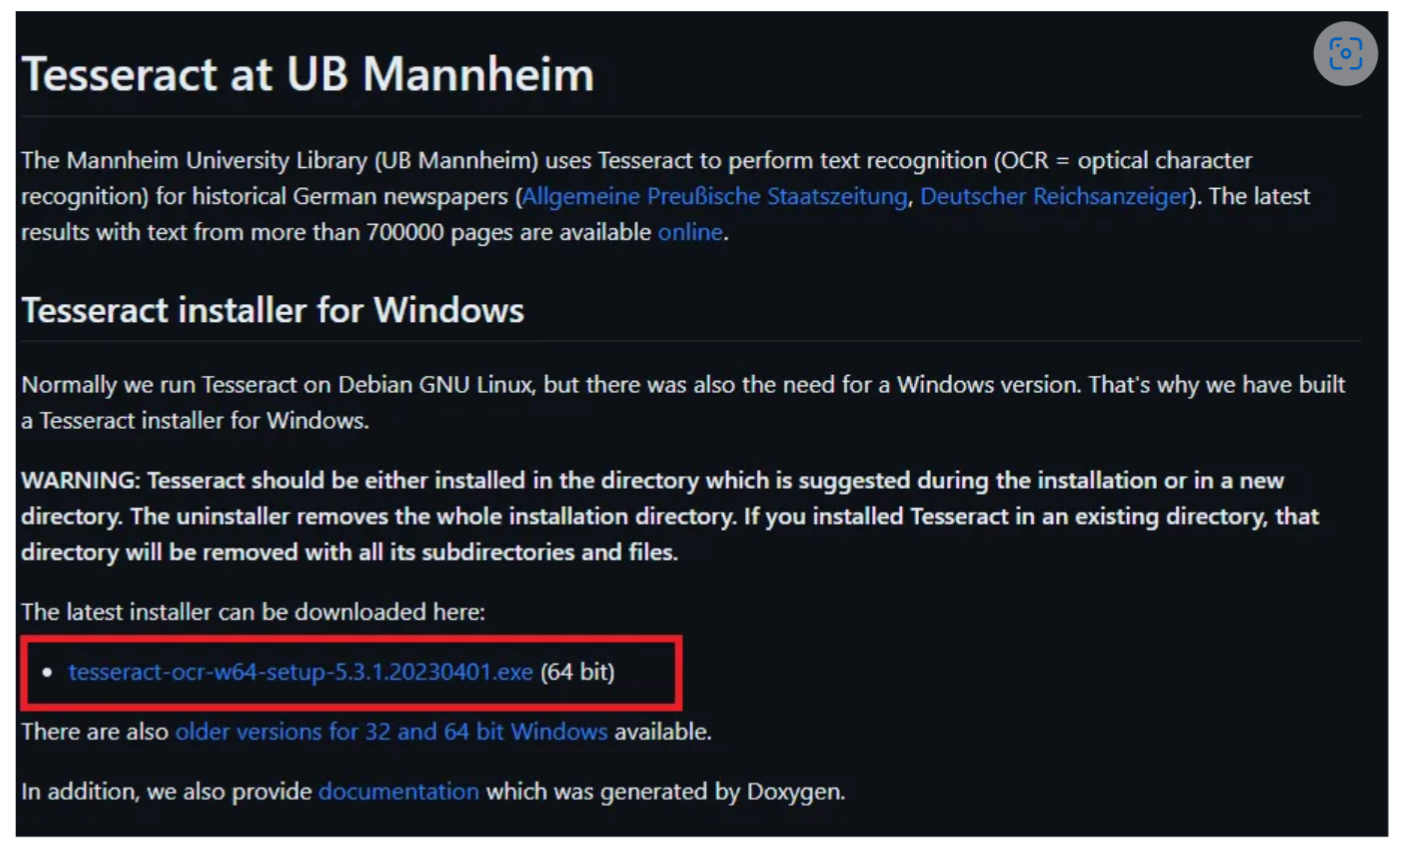
\includegraphics{Tesseract/Tesseract01}

After downloading this (.exe file), Double click and start installation.
Note: Keep the default setting and press ‘Next, Next.. and complete installation’

\section{Step 2. Install Tesseract OCR and Required Libraries}

To get started, we need to install Tesseract OCR and the necessary Python libraries. Tesseract is an open-source OCR engine maintained by Google.

For Python, we will need the following libraries:

\SHELL{pip install pytesseract}

\SHELL{pip install pillow}

\section{Step 3. Import Libraries}

    Once we have installed the required libraries, let’s import them into our Python script:

\begin{lstlisting}
import pytesseract
from PIL import image
\end{lstlisting}    
    
\section{Step 4. Define the path \SHELL{tesseract\_cmd}.}

Path \SHELL{tesseract\_cmd} might me difference in your case, To find the right path please check your directory ``tesseract installation''.

\SHELL{pytesseract.pytesseract.tesseract\_cmd = r’C:/Program Files/Tesseract-OCR/tesseract.exe’}


\section{Step 5. Load the Image}

Next, we need to load the image from which we want to extract text. Make sure the image file is in a format supported by Tesseract (e.g., PNG, JPEG, GIF). For this example, let’s assume the image file is named ``image.png'':

\begin{lstlisting}
image_path= "image.png"
image = Image.open(image.path)  
\end{lstlisting}    

\section{Step 6. Perform OCR and Extract Text}

Now that we have loaded the image, we can use pytesseract to perform OCR and extract the text from the image. The function \PYTHON{image\_to\_string} from pytesseract is used for this purpose:

\begin{lstlisting}
extracted_text = pytesseract.image_to_string(image)
\end{lstlisting}    

\section{Step 7. Post-Processing (Optional)}

Sometimes, the OCR output may contain extra spaces, line breaks, or characters that need to be cleaned up. Depending on the specific use case, you might want to perform some post-processing on the extracted text. Here’s an example of removing leading and trailing whitespaces:

\begin{lstlisting}
cleaned_text = extracted_text.strip()
\end{lstlisting}    


\section{Step 8. Display the Extracted Text}

For demonstration purposes, we’ll print the extracted text:

\begin{lstlisting}
print("Extracted Text:")
print(cleaned_text)
\end{lstlisting}    


\section{Conclusion}

We have explored the process of extracting text from images using Python. We used the pytesseract library, which serves as a Python wrapper for the powerful Tesseract OCR engine. By following the step-by-step guide and the provided Python code, you can easily extract text from images and use it for various applications in your projects.

Remember that the accuracy of the OCR output depends on factors such as image quality, resolution, and font style. Therefore, it’s essential to fine-tune the OCR process according to your specific use case and make any necessary adjustments for optimal results.


    
    
